\section{\framework Overview}

\framework is an optimization framework that takes as input a high level, architecture-independent representation of code and a set of scheduling and data mapping commands that guide code transformation.  The input can be either generated by a DSL compiler or directly written by a programmer (since the first layer of \framework{} is easy to write).  \framework{} then applies code and data layout transformations on the code and generates an architecture-specific, low-level IR that takes advantage of modern architectural features such as multicore parallelism, non-uniform memory (NUMA) hierarchies, clusters, and accelerators like GPUs and FPGAs.

\framework is designed for expressing data parallel algorithms, in particular algorithms that operate over dense arrays using loop nests and sequences of statements.  These algorithms are usually found in the areas of dense linear algebra and tensor algebra, stencil computations, image processing and deep neural networks among others.


\begin{figure}
 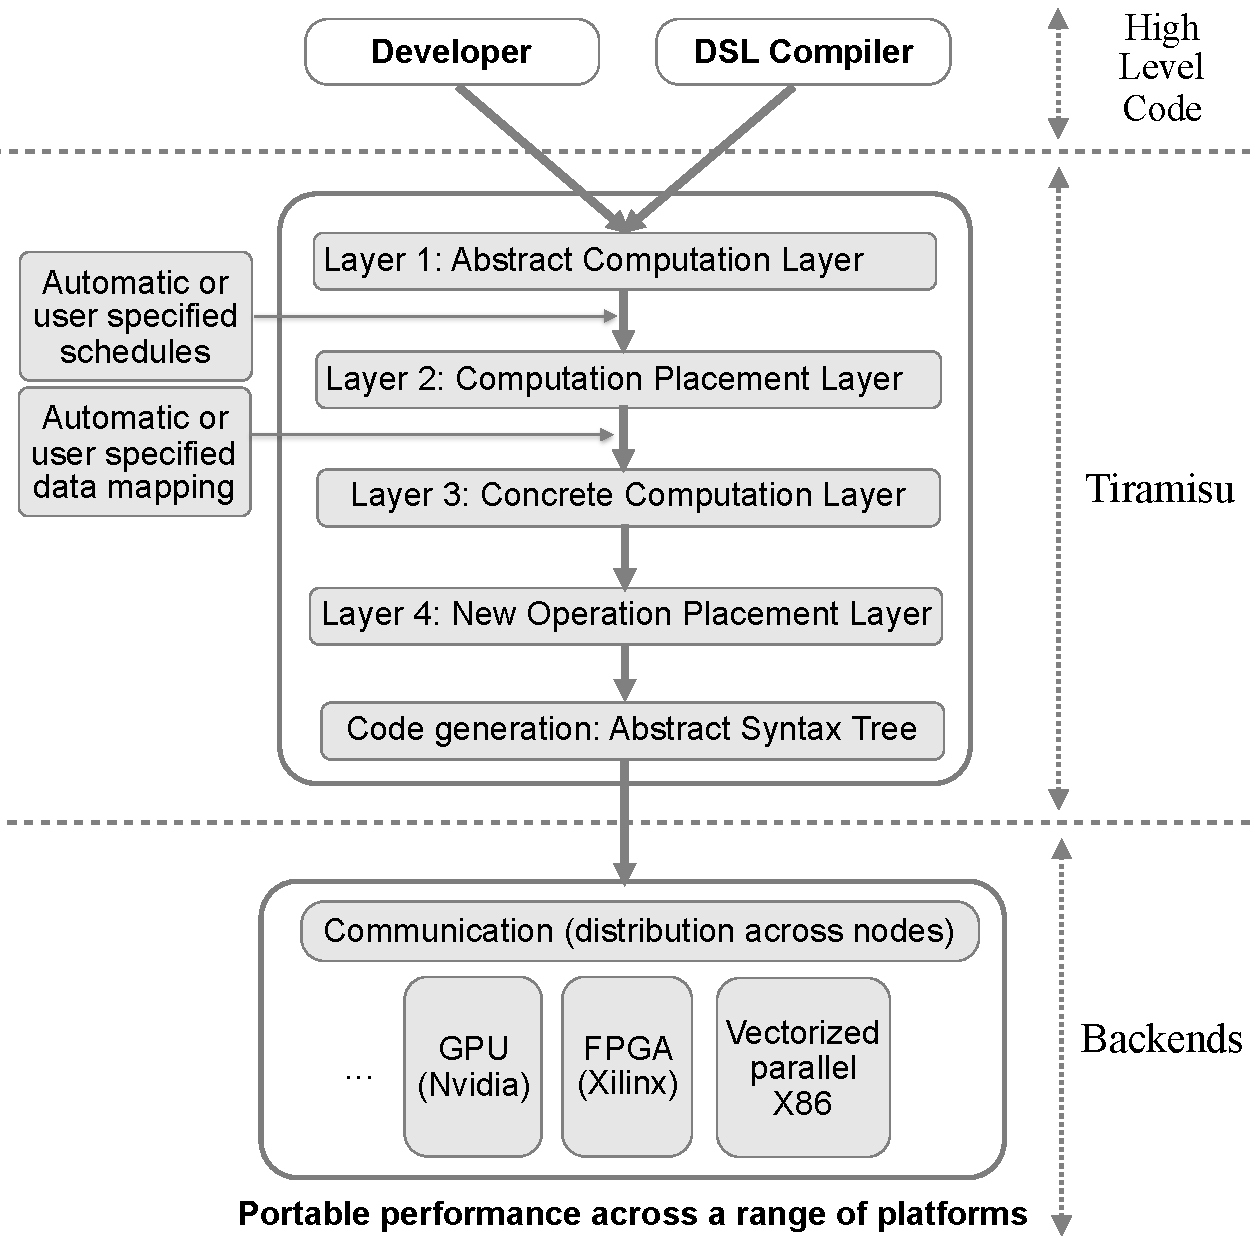
\includegraphics[scale=0.35]{./figures/fista.pdf}
 \vspace{-0.25cm}
 \caption{\framework overview}
 \label{fig:overview}
 \vspace{-0.25cm}
\end{figure}


\vspace{-0.3cm}
\subsection{The Four-Layer IR}

\framework{} uses \emph{polyhedral sets} to represent each one of the four IR layers and uses \emph{polyhedral set} and \emph{relation operations} to represent transformations on the iteration domain and data layout.  Polyhedral sets and relations are described using affine (linear) constraints over loop iterators and program parameters (invariants) and are implemented in \framework using ISL~\cite{verdoolaege_isl:_2010}.  We use a combination of classical extensions to the polyhedral model in order to support non-affine iteration spaces; these extensions are sufficient for large classes of programs in practice~\cite{benabderrahmane_polyhedral_2010,pencil}, and in particular to our areas of interest (dense linear algebra and tensor algebra, stencils, image processing and deep neural networks).

A typical workflow for using \framework is illustrated in Figure~\ref{fig:overview}.  The first layer of \framework{} can be written directly by a developer or it can be generated from a DSL compiler.  The first layer of the IR is then transformed to lower layers, and finally LLVM or other low-level IRs are generated.

The four layers of the \framework IR are:

\textbf{Layer I (\Layerone)}.
It specifies the algorithm without specifying the schedule (when and where the computations occur) or how data should be stored in memory (data layout). As there is no notion of data location, values are communicated via explicit producer-consumer relationships.

\textbf{Layer II (\Layertwo)}.
It specifies the order of execution of computations and the processor on which they execute.  This layer does not specify how intermediate values are stored in memory; this simplifies optimization passes since these passes do not need to perform complicated data-layout transformations.  The transformation of Layer I into Layer II is done automatically using scheduling and data layout commands.  Examples of the scheduling commands supported in \framework are presented in Table~\ref{tab:scheduling}.

\textbf{Layer III (\Layerthree)}.
It makes the data layout concrete by specifying where intermediate values are stored. It also adds allocation, synchronization, and communication operations.

\textbf{Layer IV (\Layerfour)}.
It specifies the schedule of operations added in Layer III (their order of execution and the processor on which they execute).

The separation into levels does not force data-layout mapping to occur after scheduling; in \framework, the user can still specify data layout before scheduling (to constrain scheduling, for example). The separation ensures that the scheduling phase can safely assume no data-layout transformations are required, greatly simplifying scheduling transformations.